\chapter{}\label{ex:aufg5}
%
\section{}\label{sec:aufg5a}
%
Die gemessene Drehzahl-Drehmomentkennlinie ist in Abb. \ref{fig:drehzahldrehmoment} dargestellt.
\begin{figure}[htb]
\centering
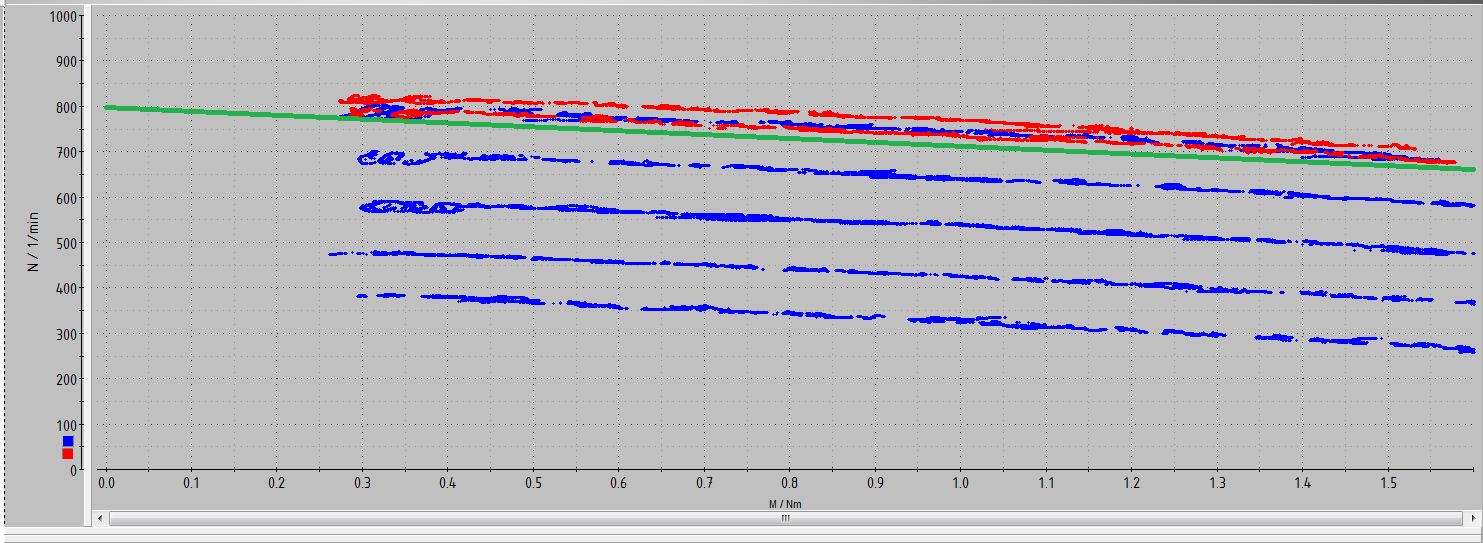
\includegraphics[width=\textwidth]{./Bilder/Drehzahl_Drehmoment_Kennlinie_inkl_Berechnet}
\caption{Drehzahl-Drehmomentkennlinienfeld}
\label{fig:drehzahldrehmoment}
\end{figure}
\section{}\label{sec:aufg5b}
%
\begin{equation}
N = \frac{U_\text{A}}{c_\text{E}\Psi} - \frac{2\pi R_\text{A}}{c_\text{E}^2\Psi^2} \cdot M_{\text{Mi}}
\end{equation}
Die eingezeichnete grüne Kennlinie in dem Kennlinienfeld Abb.\ref{fig:drehzahldrehmoment} ist die berechnete Kennlinie. Sie ist parallel verschoben, dieser Offset wird durch Ungenauigkeit des Drehmoments verursacht. Die Änderung der Steigung im Feldschwächbereich ist fast nicht zu erkennen, da das Feld nur geringfügig verringert wird.
\clearpage